\documentclass[../main.tex]{subfiles}

% MIMIC-IV, its rules, how to extract data
% Patients structure implementation


\begin{document}

In this chapter, I will detail the methodology used to extract and analyze data from the MIMIC-IV database.
The chapter is divided into three sections: Overview, dataset, and models.
The Overview section provides an overview of the proposed solution, including the main steps involved in the data extraction and analysis process.
Section dataset describes the data structure of MIMIC-IV, how the desired features were identified and  extracted in detail, including the rules for confining patients' personal data of MIMIC-IV database.
And how it leads to the implementation of a data structure that is more developer friendly dealing with patients' data.
The models section illustrates how models and the corresponding preprocessing methods are implemented to predict the risk of Acute Kidney Injury in Diabetic Ketoacidosis patients.


\section{Overview}

Overall steps of the proposed solution are shown in Figure \ref{fig:overall-steps}.
First, Diabetic Ketoacidosis (DKA) patients who were admitted to ICU are identified through International Classification of Diseases (ICD) codes and ICU stay record.
Patients with Chronic Kidney Disease (CKD) are excluded since they already have severe kidney problems and predicting AKI in these patients is not meaningful.
If a patient has multiple admissions, only the first admission is considered because of repeat sampling.
Next, with patients' identification including subject\_id, hadm\_id, and icustay\_id, other features are extracted from the MIMIC-IV database.
Many of these features changed with time, so the data is structured in a time series map where in each feature recoded time is used as key and the value is the feature value at that time.
This data structure also support retrieving the value of features as flat table for compatibility with machine learning models.
Then, the data is preprocessed and used to train predictive models of the risk of Acute Kidney Injury in DKA patients.
Finally, the models are evaluate to determine the best model and the best preprocessing method.

\begin{figure}[h]
    \centering
    \includegraphics[width=\textwidth]{Figure/Overall steps.png}
    \caption{Overall Steps}
    \label{fig:overall-steps}
\end{figure}


\section{Dataset}

In this section, we will dive into the MIMIC-IV database to understand its structure and identify relevant features then establish a data structure that is more developer friendly dealing with patients' data.


\subsection{MIMIC-IV analysis}
\label{subsec:MIMIC-IV-analysis}

In order to successfully predict the risk of AKI in DKA patients, it is crucial to extract patients' health record from the MIMIC-IV database.
Thus, the first step is to understand the structure of the MIMIC-IV database and identify the features that are relevant to the prediction of AKI in DKA patients.
The tree structure of MIMIC-IV is shown in Figure \ref{fig:mimic-iv-structure}.

MIMIC-IV is a large, freely-available database comprising de-identified health-related data associated with over 300.000 distinct patients who were admitted to critical care units.
It is separated into 2 main categories: hospital data and ICU data.

\begin{figure}[h]
    \centering
    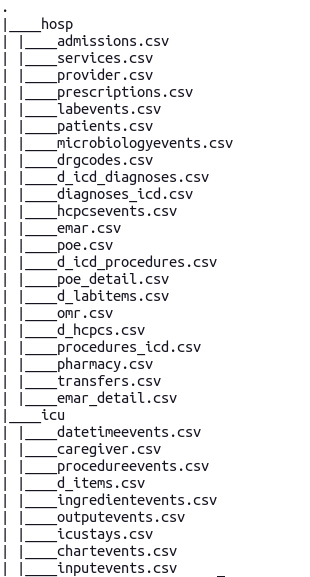
\includegraphics[width=0.5\textwidth]{Figure/MIMIC-IV_tree.png}
    \caption{MIMIC-IV structure}
    \label{fig:mimic-iv-structure}
\end{figure}


\subsubsection{Hospital data}

Hospital data stores information about patients' admission, basic information, result of laboratory tests, patients' diagnosis, and other general information.
Looking deeper into the hospital data, we can see that it is divided into several tables, each of which stores different types of information.
It is easy to notice that there are some table with "d\_" prefix, which means that these tables store definitions of the data in other tables.

For example, in "d\_icd\_diagnoses" table, we can find information about the International Classification of Diseases (ICD) codes, representing in columns: icd\_code, icd\_version, long\_title.
This table describes respectively the code for the diagnose, the version of the code (currently in MIMIC-IV, both version 9 and 10 are supported) and finally the description of the the diagnosis which is its technical name.
Its code and version are referred in the other table like "diagnoses\_icd" table to mark patients with positive diagnosis of the disease.
Thank to them, I could find the ICD codes for DKA and CKD to identify patients with DKA and exclude patients with CKD.

With "d\_icd\_procedures" table, we can find information about which procedures were performed on patients, representing in columns: icd\_code, icd\_version, long\_title.
It is very helpful to determine the interventions that were performed on patients, which could affect the risk of AKI in DKA patients.

In "d\_labitems" table, we can find information about the laboratory tests that were performed on patients, representing in columns: itemid, label, fluid, category. Column "itemid" is the unique identifier for each laboratory test and will be referred by other tables like "labevents" table to store the result of the test for each patients. Other columns are the label or name of the test, the fluid that was tested (e.g. blood, urine, etc.), and the category of the test (e.g. chemistry, blood gas, etc.).
As laboratory tests contains many important features used in predicting the risk of AKI in DKA patients, this table helps in identify the itemid of the tests that are relevant to the prediction.

Table "d\_hcpcs" stores information about the Healthcare Common Procedure Coding System (HCPCS) codes, representing in columns: hcpcs\_code, short\_description, long\_description.
This table functions similarly to the "d\_icd\_procedures" table, but it uses HCPCS standard which is primarily used in the United States of America.

The remaining tables in the hospital data store information associated with individuals.
Thus, they commonly include "subject\_id" column, which is an unique identifier for each patient and "hadm\_id" column - an unique identifier for each hospital admission.

In "admissions" table, we can find information about patients' admission, representing in columns: subject\_id, hadm\_id, admittime, dischtime, deathtime, admission\_type, admit\_provider\_id, admission\_location, discharge\_location, insurance, language, marital\_status,race,edregtime,edouttime,hospital\_expire\_flag.
Column "admittime" is the time when the patient was admitted to the hospital,
"dischtime" is the time when the patient was discharged from the hospital,
"deathtime" is the time when the patient died (this date were collected 2 years after the last patients recoded got discharged from the hospital),
"admission\_type" is the type of admission (e.g. URGENT, OBSERVATION ADMIT, etc.),
"admit\_provider\_id" is the identifier of the provider who admitted the patient and could be found in "provider" table,
"admission\_location" and "discharge\_location" are the medical facility where the patient was admitted and was discharged,
"insurance" is the type of insurance the patient has,
"language" is the language spoken by the patient,
"marital\_status" is the marital status of the patient.
In this table, I focus mostly on "admittime" and identified columns to match DKA-ICU cases with the corresponding demographic features.

Table "labevents" stores information about the laboratory tests that were performed on patients, representing in columns: labevent\_id, subject\_id, hadm\_id, specimen\_id, itemid, order\_provider\_id, charttime, storetime, value, valuenum, valueuom, ref\_range\_lower, ref\_range\_upper, flag, priority, comments.
Column "labevent\_id" is the unique identifier for each laboratory test, and "itemid" is the reference to "d\_labitems" table.
The time when the test was performed and stored in hospital databases can be found in "charttime" and "storetime".
Both "value" and "valuenum" is the result of the test. It is documented that "value" is the more readable representation of the result while "valuenum" is the numerical value.
The remaining columns are used in medical and monitoring purposes. 

Patients' encoded information are stored in "patients" table, representing in columns: subject\_id, gender, anchor\_age, anchor\_year, anchor\_year\_group, dod.
The anchor\_year is a deidentified year occurring sometime between 2100--2200, and the anchor\_year\_group is a three year long date ranges between 2008--2019. 
These pieces of information allow researchers to infer the approximate year a patient received care.
For instance, if a patient's anchor\_year is 2158, and their anchor\_year\_group is 2011--2013, then any hospitalizations for the patient occurring in the year 2158 actually occurred sometime between 2011--2013. 
Finally, the anchor\_age provides the patient age in the given anchor\_year. 
If the patient was over 89 in the anchor\_year, this anchor\_age has been set to 91 regardless of the actual age of the patient.
To calculate the actual age of the patient, the following formula can be used: 

\begin{equation}
    actual\_age = anchor\_age + anchor\_year - anchor\_year\_group
\end{equation}

Diagnose information are stored in "diagnoses\_icd" table, representing in columns: subject\_id, hadm\_id, seq\_num, icd\_code, icd\_version. 
By referencing table "d\_icd\_diagnoses", we can find the description of the diagnose by the code and version and identify who has DKA and CKD stage 5.


% other unrelated tables 
% services, provider, prescription, microbioevent, drgcodes, hpcpevent, emar, poe, poe_detail, omr, pharmacy, transfer, emar_detail,  

The rest of hospital tables store information for billing and controlling purposes so they are not delved deeply in this thesis.
For example, table "services" stores information about the services that were provided to patients, representing in columns: subject\_id, hadm\_id, transfertime, prev\_service, curr\_service. 
And "provider" has a single column "provider\_id" which is the unique identifier for each provider.
Table "prescription" provides data related to prescriptions issued to patients, including medication details (name, dosage, frequency), prescribing physician, and date/time of prescription.
Details of microbiology test results, including microorganisms identified, antibiotic sensitivity results, and other relevant microbiological data are stored in "microbioevent".
Table "dgrcodes" or Diagnosis-related group codes contains codes assigned to patients for billing and classification purposes, indicating the type of treatment received.


\subsubsection{Intensive Care Unit data}

ICU data includes information about patients during their stay in the ICU, including vital signs, medications, interventions, and other information that is recorded promptly.

Like hospital data, ICU data also contains definition table named "d\_items" which stores information about the items that are recorded in the ICU stored in other tables. 
In this table, we can find 9 columns: itemid, label, abbreviation, linksto, category, unitname, param\_type, lownormalvalue, highnormalvalue.
Column "label" is the name of the item and "abbreviation" keeps the short name of it.
Table which the measurements of the item is stored is specified in "linksto".
With "unitname", we can convert same measurement in different unit one unified unit.
The rest of columns are not in the scope of the thesis so they are not discussed here.

Table "chartevents" stores information about the measurements that were recorded in the ICU, representing in columns: subject\_id, hadm\_id, stay\_id, caregiver\_id, charttime, storetime, itemid, value, valuenum, valueuom, warning.
Column "itemid" is the reference to "d\_items" table allowing us to find the name of the item.
"Valueuom" indicates the unit of the measurement, and "value" and "valuenum" are respectively string representation and number the result of the measurement.
Most of vital signs come from this table contributing to the detection of organs failure.
% Add other columns if needed.

In "outputevents" and "inputevents" table, we can find information about the input and output of patients which is important in evaluate the kidney function.
For instance, a drastic change in urine output could be a sign of kidney failure.


\subsection{Storage structure and data extraction}

Since my main contribution lies in taking the fluctuating values of patients' features over time into account, I have designed a data structure that is capable of grouping and keeping measured values in time-respected order.
Each patient is represented as an object Patient shown in the code below \ref{lst:Patient}.

\begin{lstlisting}[language=Python, caption={class Patient}, label={lst:Patient}]
    
class Patient:
    
    def __init__(
        self,
        subject_id: int,
        hadm_id: int,
        stay_id: int,
        intime: str | datetime | datetime64 | Timestamp,
        measures: Dict[str, Dict[Timestamp, float] | float]
    ) -> None:
        self.subject_id = subject_id
        self.hadm_id = hadm_id
        self.stay_id = stay_id
        self.intime = to_datetime(intime)
        self.measures: Dict[str, 
            Dict[Timestamp, float] | float] = SortedDict()

\end{lstlisting}

In this class, the patient is identified by subject\_id, hadm\_id, and stay\_id and "intime" signifies the time when the they were admitted to the ICU.
The "measures" attribute is a dictionary where patient's demographic, laboratory tests, vital signs and other features are stored with their name as key and value is either a single value for features like age, stage of comorbidities, or a dictionary if the features changed over time i which the key is the time when the measurement was taken and the value is the measurement itself.
This class also supports the retrieval of the value of a feature at a specific time, which is useful for machine learning models that require a flat table as input.

\begin{lstlisting}[language=Python, caption={getMeasuresBetween method}, label={lst:getMeasuresBetween}]

(method) def getMeasuresBetween(
    self: Self@Patient,
    fromTime: Timedelta,
    toTime: Timedelta,
    how: str | ((DataFrame) -> float) = "avg",
    getAkiRealTime: bool = False,
    measureTypes: Literal['all', 'static', 'time'] = "all"
) -> DataFrame

\end{lstlisting}

The method getMeasuresBetween \ref{lst:getMeasuresBetween} is used to retrieve the value of features in a time range compared to patient's intime.
The method takes 4 arguments: fromTime and toTime are the time range, "how" is the method to aggregate the values in the time range if more than one exist, getAkiRealTime is a flag to also return AKI status in the returned DataFrame, finally, measureTypes is the type of features to retrieve which is helpful for models that can process static and time series features separately.
Parameter "how" can be a string that represents predefined method to aggregate the values in the time range or a function that takes a DataFrame of value and time and returns a single value.
Currently, the predefined methods are "first" and "last" for the first and last value according to recorded time, " "avg" for average, "std" for standard deviation, "max" for maximum, and "min" for minimum.
It is also worth noting that the "measures" attribute is a SortedDict which allow this method to run binary search in O(log(n)) time complexity.

This class is also a place gathering all features extracted from MIMIC-IV database with class method "loadPatients".
When this method is called, it will first establish a list of target patients by identifying patients with DKA and detect in them if they got admitted to Intensive Care Unit (ICU).
This step is done by matching the ICD codes of their hospitalizations with that represent DKA then searching for their hadm\_id in the ICU data, the existence of stay\_id in the ICU data indicates that the patient was admitted to the ICU.
These patients would be delivered to next filtering step where patients with CKD stage 5 are excluded from the list because not only did the damage caused to their kidneys is already severe and predicting AKI in these patients is not meaningful but also their indicators show a heavy similarity to AKI patients.
Thus, adding these patients potentially raise the noise in dataset and damage the model's performance.
After this step, I found 1213 patients with DKA and not CKD stage 5.
Then, I evaluate patient data during ICU according to \citetitle{kdigo-aki-guideline} \cite{kdigo-aki-guideline} to determine the AKI status of each patient.
There are 476 patients who is diagnosed with AKI during their ICU stay, or 39.24\% of the target patients.
Finally, this method run sql queries to extract the features from the database.
For instance, to get urine output of a patients, the following query is used \ref{lst:SQL-urine-output}.

\begin{lstlisting}[language=SQL, caption={SQL query to get urine output}, label={lst:SQL-urine-output}]

    WITH uo AS (
    SELECT oe.stay_id,
        oe.charttime,
        CASE
            WHEN oe.itemid = 227488
            AND oe.value > 0 THEN -1 * oe.value
            ELSE oe.value
        END AS urineoutput
    FROM outputevents AS oe
    WHERE itemid IN (
            226559
            /* Foley */
,
            226560
            /* Void */
,
            226561
            /* Condom Cath */
,
            226584
            /* Ileoconduit */
,
            226563
            /* Suprapubic */
,
            226564
            /* R Nephrostomy */
,
            226565
            /* L Nephrostomy */
,
            226567
            /* Straight Cath */
,
            226557
            /* R Ureteral Stent */
,
            226558
            /* L Ureteral Stent */
,
            227488
            /* GU Irrigant Volume In */
,
            227489
            /* GU Irrigant/Urine Volume Out */
        )
    )
    SELECT stay_id,
        charttime,
        SUM(urineoutput) AS urineoutput
    FROM uo
    GROUP BY stay_id,
        charttime;

\end{lstlisting}

From this query \ref{lst:SQL-urine-output}, it is clear that the urine output is calculated by summing the output of different types of catheters and stents with an exception "GU Irrigant Volume In" which is negated to represent the output.
As shown in the previous subsection \ref{subsec:MIMIC-IV-analysis}, the itemid of each measure can be found in "d\_items" table.
Other features are extracted in a similar way and stored in the "measures" attribute of the Patient object.


\section{Models}

In this section, I will describe the models used to predict the risk of Acute Kidney Injury in Diabetic Ketoacidosis patients and the preprocessing methods used to prepare the data for these models.
The preprocessing methods are separated into two main categories: tabular-based models and time series-based model.
However, in both categories, reducing missing values is crucial and is achieved in a same way in this thesis.
First, the features which have more than 20\% missing values are removed.
Then, patients with more than 20\% missing values are also removed.
This is to guarantee that after split train-test, the test set still has all features used to train the model.
This process excluded nine features and three patients from the dataset proposed by \citeauthor{xgboost-aki-dka} \cite{xgboost-aki-dka}.
As one of contributions in this thesis, I added nine features that is commonly measured in target patients leading to the exclude of 6 more patients.

Both datasets are evaluated in same ways to determine if the newly added features are useful in predicting the risk of AKI in DKA patients.
The remaining missing values are either left to be Not-a-Number (NaN), filled with zeros or filled using K-Nearest Neighbors (KNN) algorithm.
We then evaluate which method is the most suitable option for each model.


\subsection{Tabular-based models}

Since the amount of target patients is not large, it is more reasonable to cross validate on the whole population.
The dataset is split into 5 roughly equal parts of 241-242 patients.
The I iteratively train the model on 4 parts and evaluate on the remaining part.
In each iteration, the four training parts are grouped and then using method "getMeasuresBetween" \ref{lst:getMeasuresBetween} to get the table data of the time range 24 hours from the patient's intime.
Each strategy of aggregate multiple values in the time range is evaluated to determine the best method for predicting AKI in DKA-ICU patients.
The values are then filtered to remove outlines using the following formula:

\begin{equation}
    \begin{aligned}
        Q1 - 1.5 \times IQR &\leq x \leq Q3 + 1.5 \times IQR \\
        where: \\
        Q1 &= \text{first quartile} \\
        Q3 &= \text{third quartile} \\
        IQR &= Q3 - Q1
    \end{aligned}
\end{equation}
Here, the first quartile is the median of the lower half of the data, the third quartile is the median of the upper half of the data, and the interquartile (IQR) range is the difference between the third and first quartile.
The values that are outside of this range are considered as outlines and are removed from the dataset.
The categorical features are then one-hot encoded and the numerical features are standardized Eq.\ref{eq:standardized}.

\begin{equation}
    \label{eq:standardized}
    \begin{aligned}
        x_{\text{standardized}} &= \frac{x - \mu}{\sigma} \\
        where: \\
        \mu &= \text{mean of the feature} \\
        \sigma &= \text{standard deviation of the feature}
    \end{aligned}
\end{equation}
The features are then used to train the model and evaluate the model's performance using the area under the receiver operating characteristic curve (AUC-ROC).
The average AUC-ROC of the 5 iterations is then calculated to determine the best preprocessing method for the tabular-based models.

For each model, four instances are trained: one with missing values left as NaN or zeros, one with missing values filled by KNN; in the other two, training data is further split into training and validation set to tune the hyperparameters of the model.
In validate cases, the training set is split again into 5 parts and the model is trained on 4 parts and evaluated on the remaining part.
This creates 5 models which are wrapped in a voting layer that used median of the predictions to make the final prediction.
The model is then evaluated on the test set to compete with the other models.

\begin{figure}[h]
    \centering
    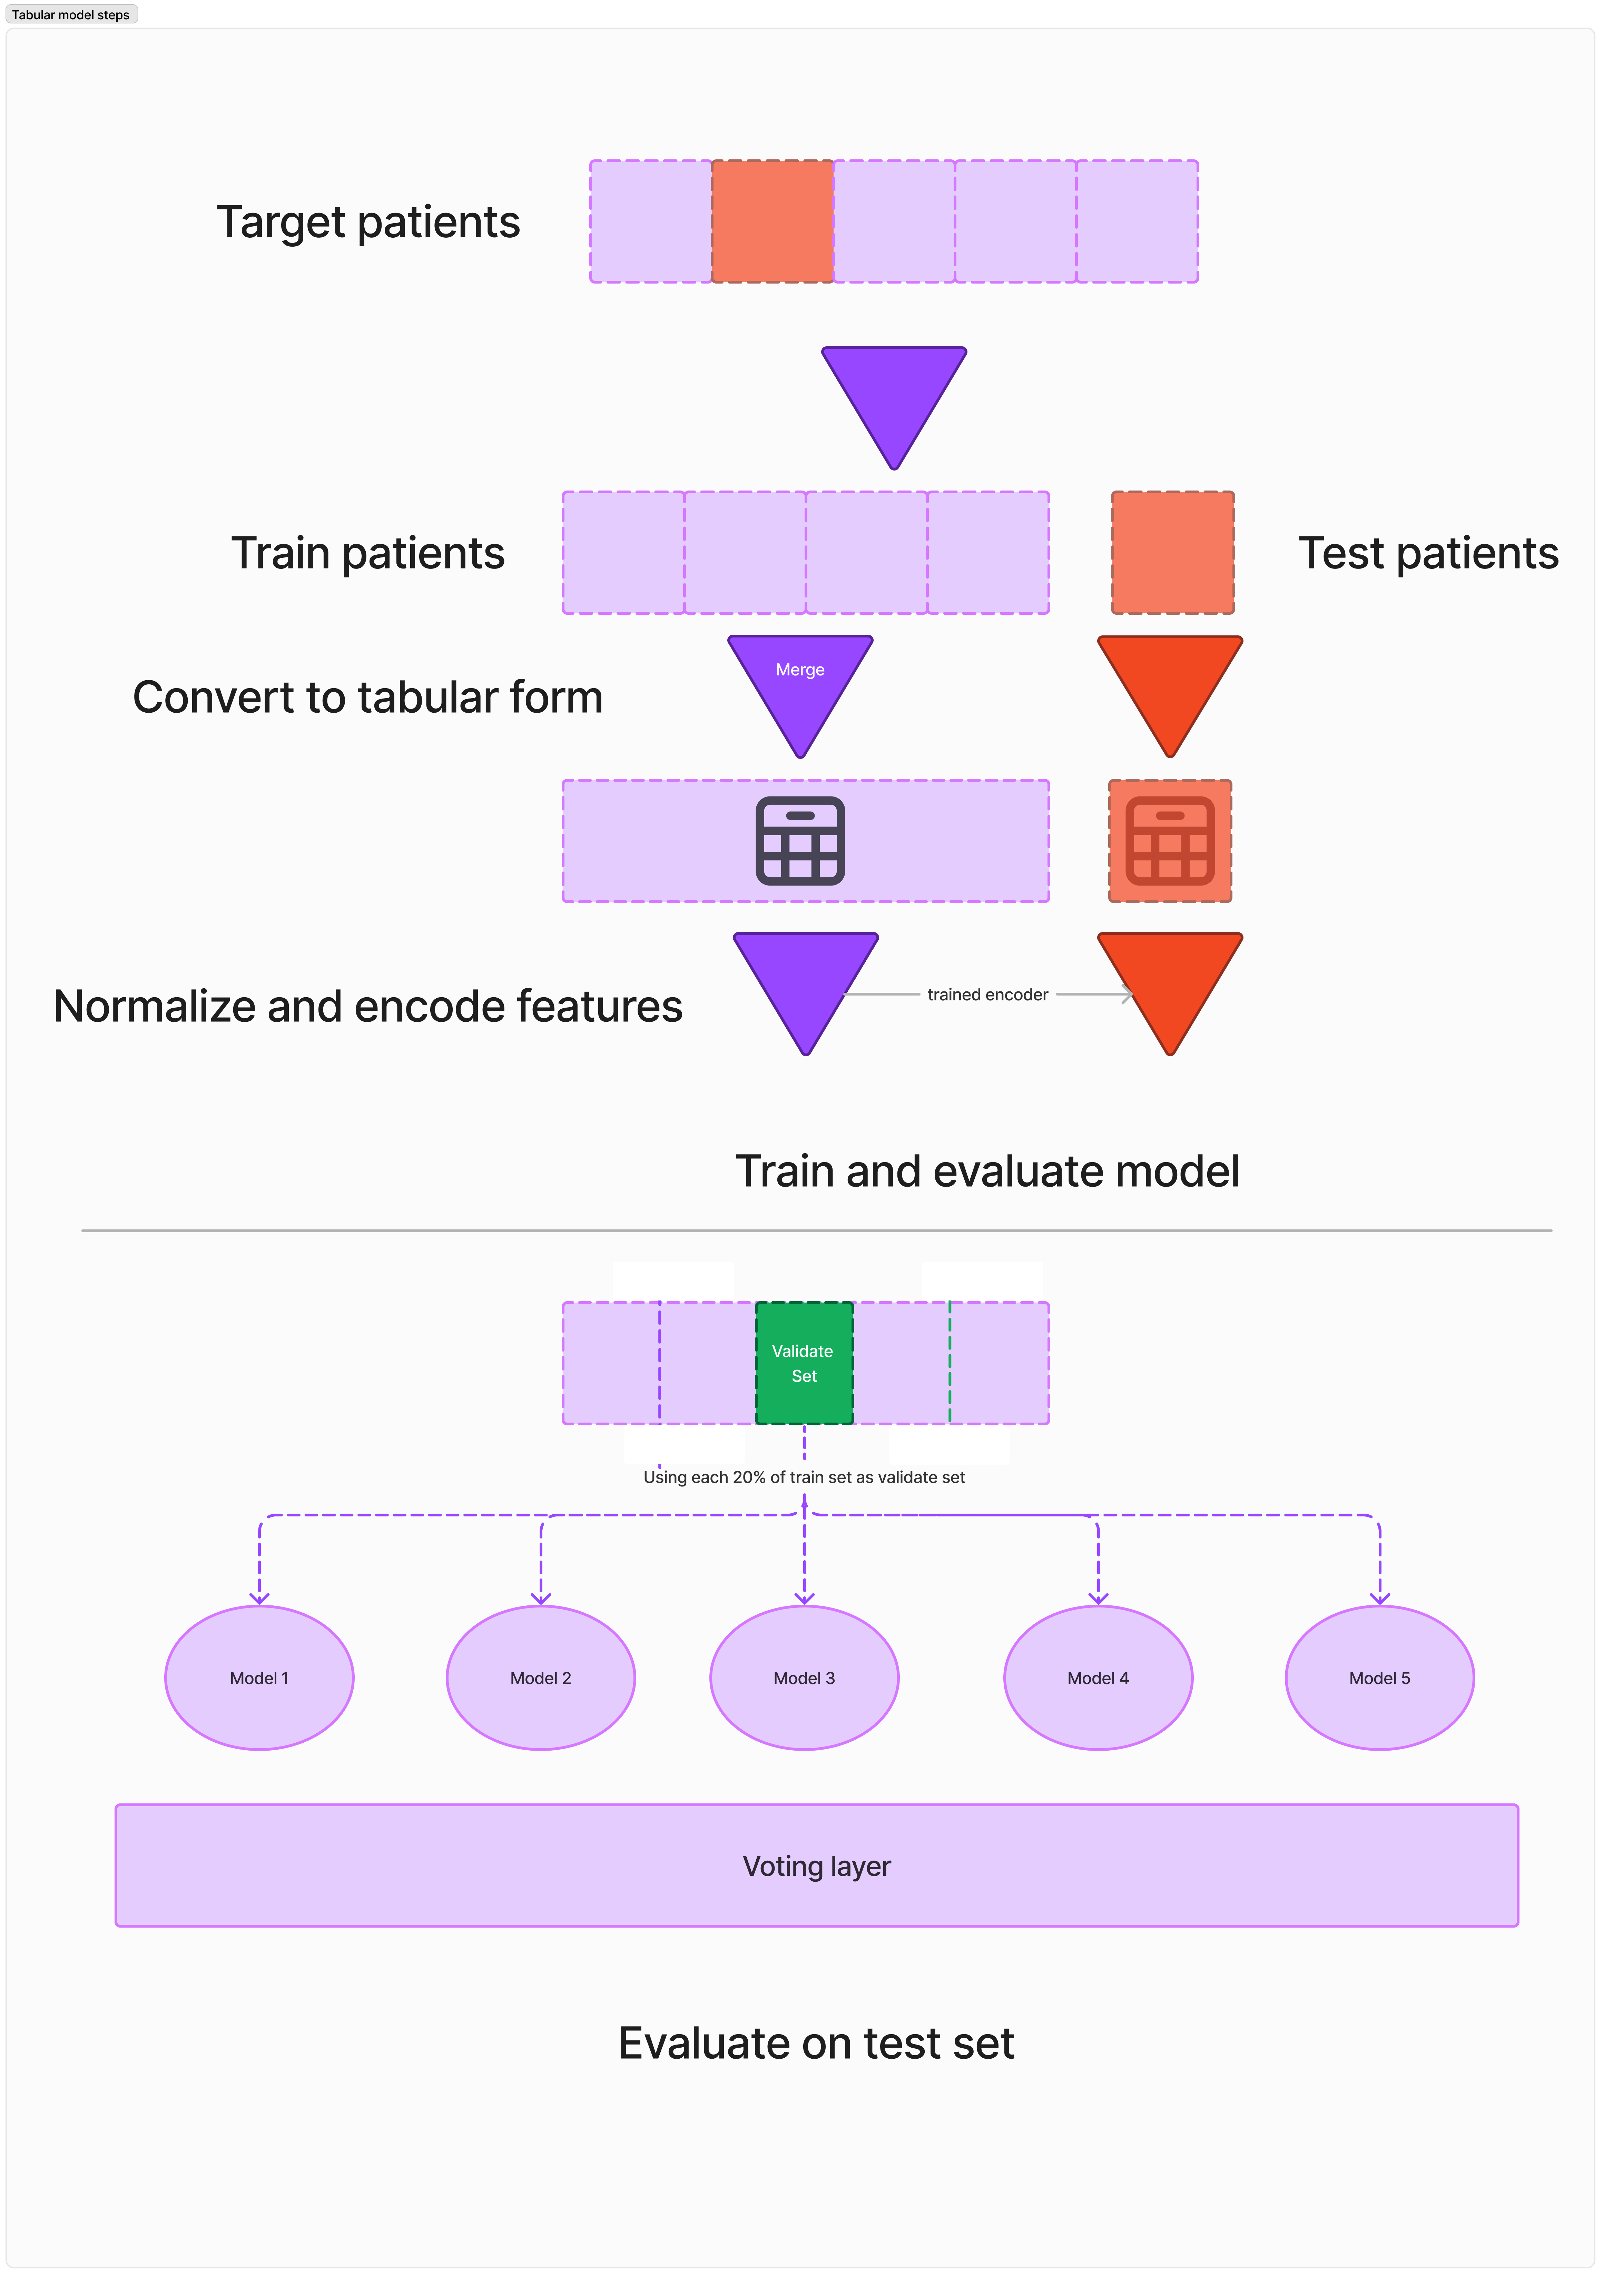
\includegraphics[width=0.8\textwidth]{Figure/Tabular Steps.png}
    \caption{Prepare data steps for tabular based predictive models, second iteration}
    \label{fig:tabular-steps}
\end{figure}

One of the iteration of the tabular-based models is shown in Figure \ref{fig:tabular-steps} where the second part is chose as test set.
The four remaining parts are grouped and the data is prepared as described above to produce a training DataFrame and a test DataFrame.
The training DataFrame is then when through preprocessing steps as mentioned above where outlines is determined and removed, categorical features are one-hot encoded, and numerical features are standardized.
It is worth noting that the test DataFrame is supposed to not know at the time of training so its outlines and encoders are determined by the training DataFrame instead.
For training process with validation, it is shown in the Figure \ref{fig:tabular-steps} that the training DataFrame is split into 5 parts and is iteratively used to train five models.
Which are stayed behind a voting layer to make the final prediction. 


In this thesis, I will evaluate the performance of the following tabular-based models: XGBoost \cite{xgboost-source}, GRANDE \cite{GRANDE-source}, and TabPFN\cite{tabpfn}.


\begin{figure}[h]%&= \text{mean of the feature} \\
    \centering
    \begin{subfigure}{0.8\textwidth}
        \centering
        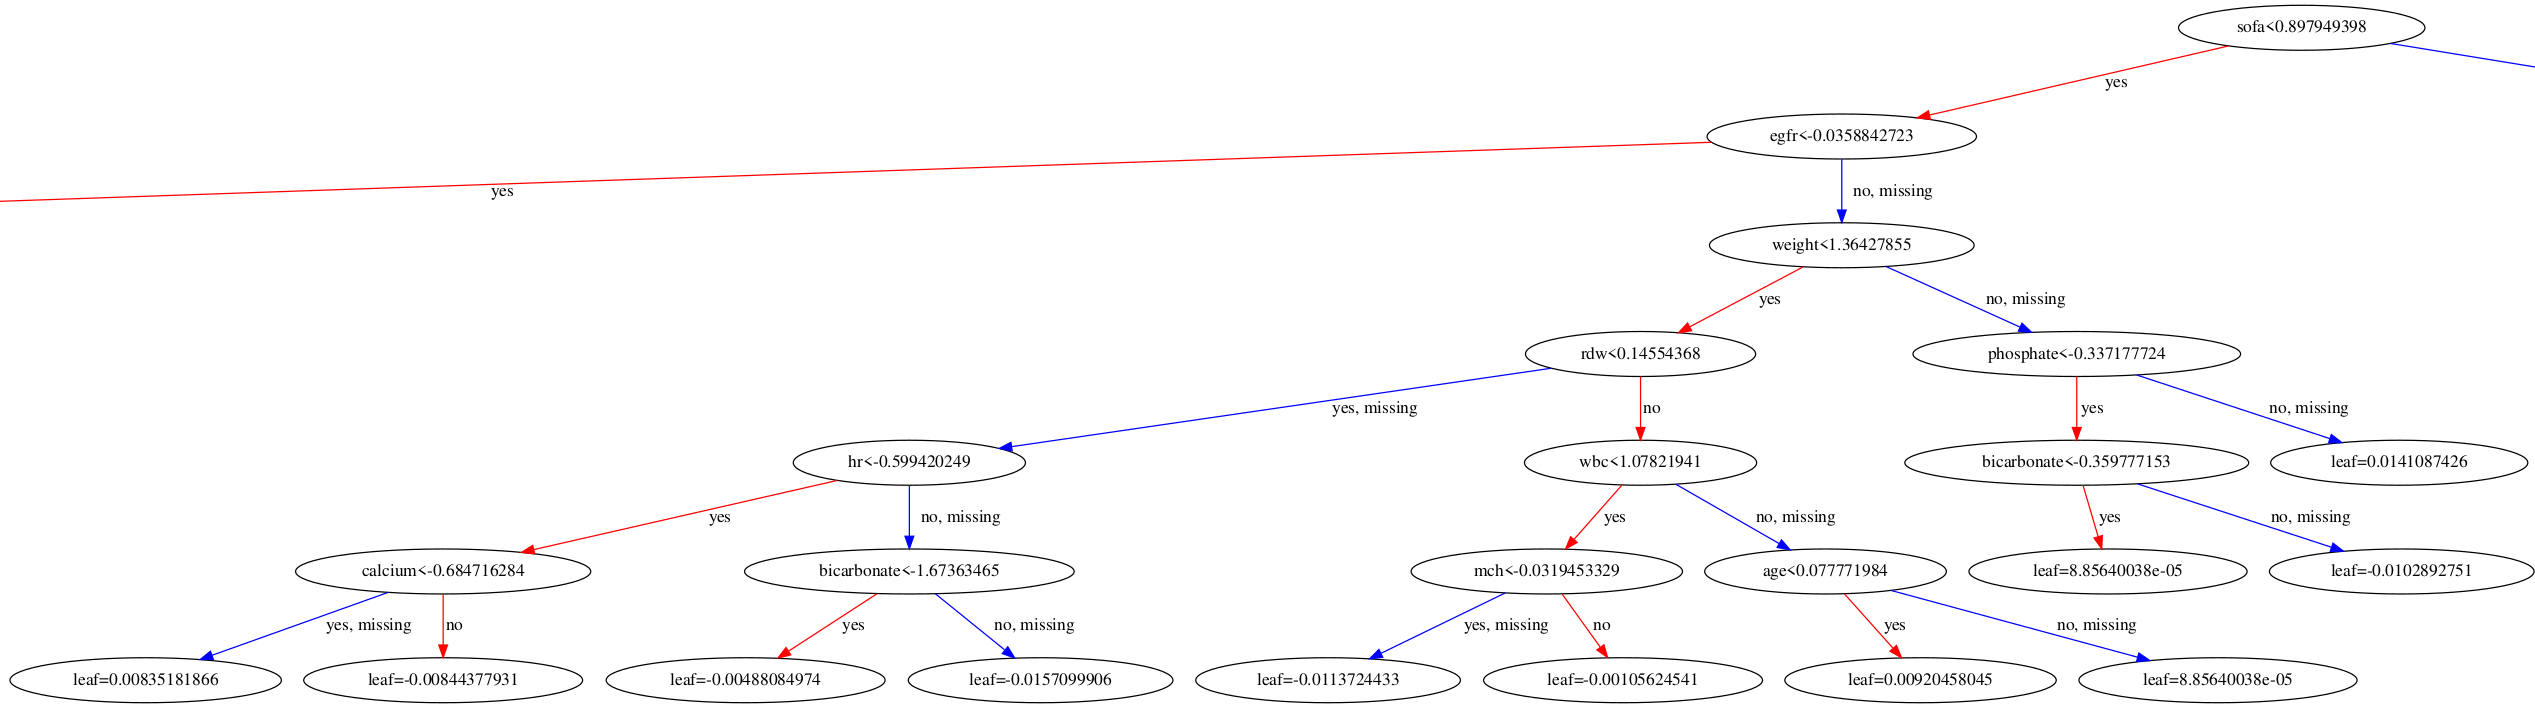
\includegraphics[width=\linewidth]{Figure/xgb_tree_high_quality-mid.png}
        \caption{Middle part of the decision tree}
        \label{fig:image1}
    \end{subfigure}
    \hfill
    \begin{subfigure}{0.8\textwidth}
        \centering
        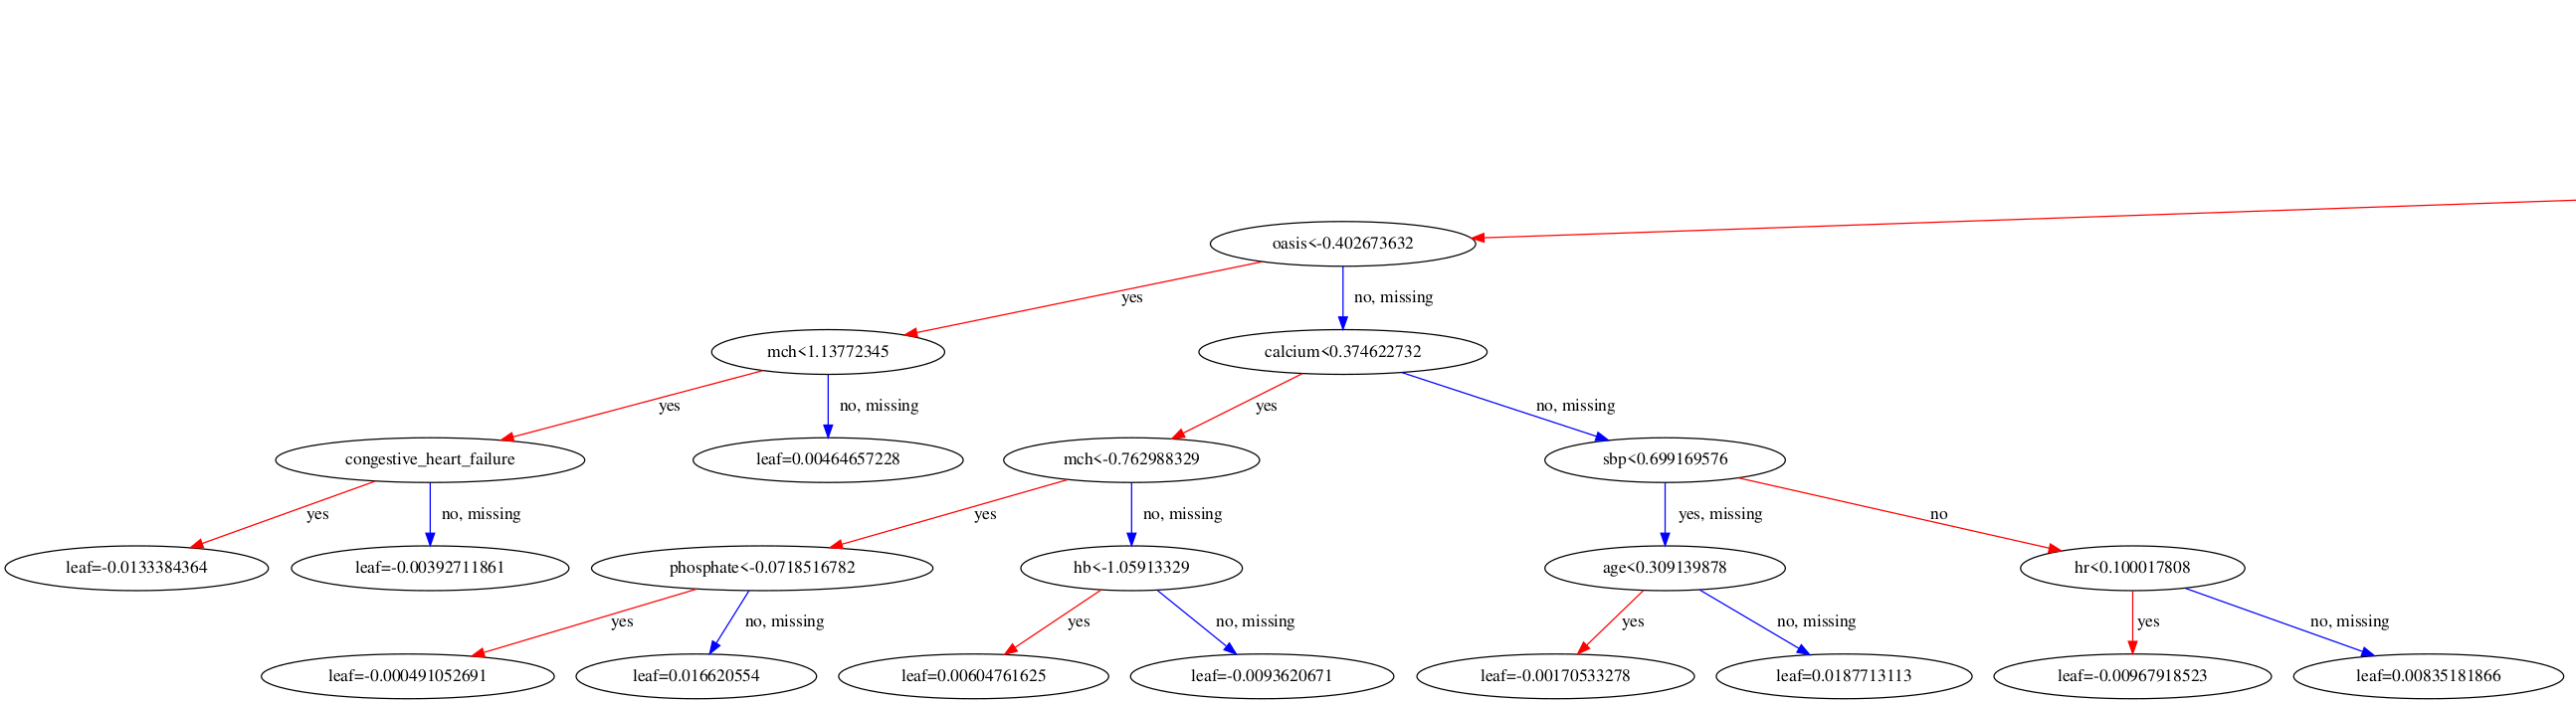
\includegraphics[width=\linewidth]{Figure/xgb_tree_high_quality-left.png}
        \caption{Left side of the decision tree}
        \label{fig:image2}
    \end{subfigure}
    \hfill
    \begin{subfigure}{0.8\textwidth}
        \centering
        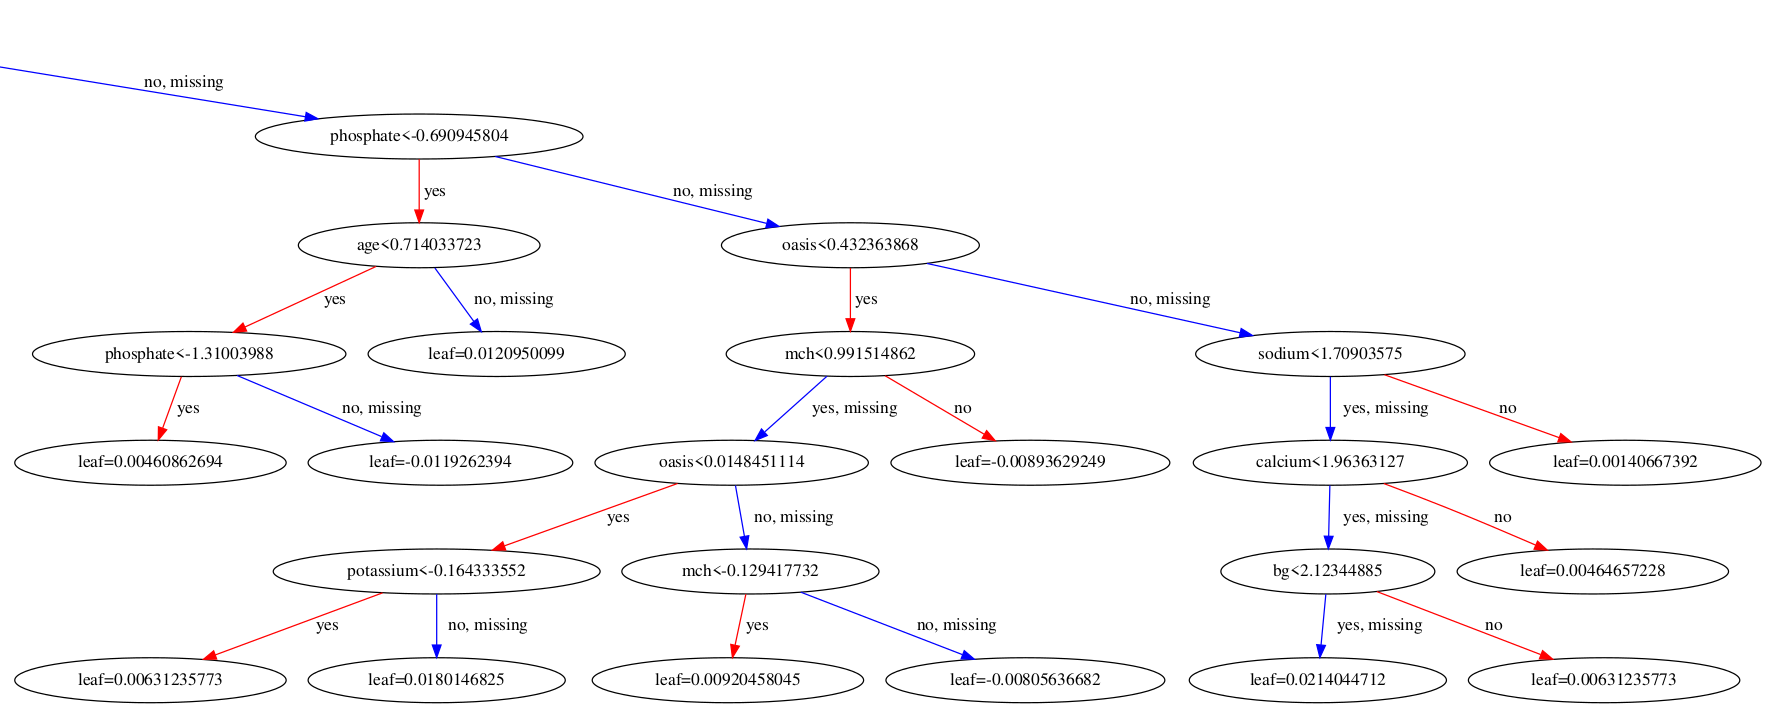
\includegraphics[width=\linewidth]{Figure/xgb_tree_high_quality-right.png}
        \caption{Right side of the decision tree}
        \label{fig:image3}
    \end{subfigure}
    \caption{XGBoost decision tree}
    \label{fig:xgboost-tree}
\end{figure}

\begin{table}
    \centering
    \begin{tabular}{|l|l|}
        \hline
        \textbf{Feature} & \textbf{Importance} \\ \hline\hline
        weight & 412.0 \\ \hline
        plt & 260.0 \\ \hline
        rbc & 253.0 \\ \hline
        wbc & 240.0 \\ \hline
        preiculos & 237.0 \\ \hline
        oasis & 232.0 \\ \hline
        mch & 230.0 \\ \hline
        age & 229.0 \\ \hline
        rdw & 213.0 \\ \hline
        bg & 209.0 \\ \hline
        sbp & 208.0 \\ \hline
        egfr & 208.0 \\ \hline
        saps2 & 202.0 \\ \hline
        phosphate & 196.0 \\ \hline
        sofa & 190.0 \\ \hline
        hr & 186.0 \\ \hline
        hematocrit & 181.0 \\ \hline
        mchc & 180.0 \\ \hline
        scr & 177.0 \\ \hline
        calcium & 177.0 \\ \hline
        chloride & 161.0 \\ \hline
        potassium & 155.0 \\ \hline
        dbp & 147.0 \\ \hline
        bun & 147.0 \\ \hline
        mcv & 146.0 \\ \hline
        hb & 136.0 \\ \hline
        sodium & 135.0 \\ \hline
        rr & 131.0 \\ \hline
    \end{tabular}
    \caption{Feature importance of XGBoost model}
    \label{tab:xgboost-feature-importance}
\end{table}


\begin{figure}
    \centering
    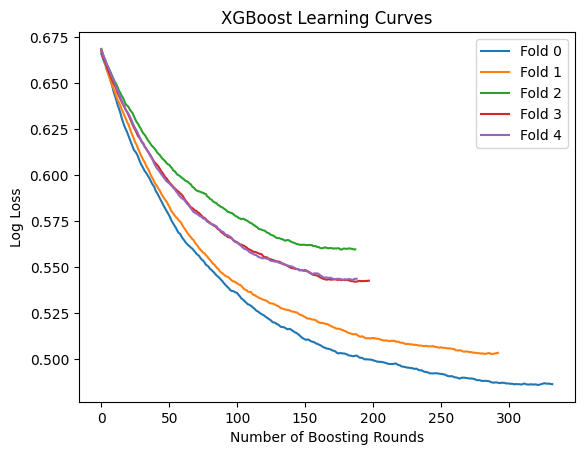
\includegraphics[width=0.8\textwidth]{Figure/xgb-learning-curve.png}
    \caption{XGBoost learning curve on the 5 iterations}
    \label{fig:xgboost-learning-curve}
\end{figure}

XGBoost is a popular machine learning algorithm that is used for regression and classification problems, especially in the field of healthcare because it can handle missing values and is less prone to overfitting.
It has been state-of-the-art in many medical prediction studies, just to name a few: \citetitle{other-xgboost-aki}, \citetitle{other-xgboost-mimic} or \citetitle{other-xgboost-mimic-2}.
the XGBoost algorithm is used as a baseline to verify that my target patients are aligned with the dataset proposed by \citeauthor{xgboost-aki-dka} \cite{xgboost-aki-dka} without a large performance gap.
The algorithm draws series of decision trees to predict the target variable and each tree is assigned a weight based on its performance.
Shown in Figure \ref{fig:xgboost-tree} is a decision tree of the XGBoost algorithm.
We can also see the feature importance of the XGBoost model in Table \ref{tab:xgboost-feature-importance} and the learning curve of the model in Figure \ref{fig:xgboost-learning-curve}.


Designed in \citeyear{GRANDE-source} by \citeauthor{GRANDE-source} \cite{GRANDE-source}, GRANDE tackled a gap in tabular-based models prediction with deep learning models.
It is a deep learning model that excels in handling heterogeneous datasets often found in applications like medical diagnosis.
Unlike traditional tree-based models that may struggle with the diverse challenges of tabular data, such as missing values, class imbalance, and mixed feature types, GRANDE leverages end-to-end gradient descent to optimize hard, axis-aligned decision trees within an ensemble framework.
One interesting note about GRANDE is that it requires validate data so in this case, the two no-validate methods are not used.


Aside from gradient-based models, TabPFN is a deep learning model that uses a Bayesian approach to clear the relations between features and the target variable.
The result of relationships founded can be seen in Figure \ref{fig:tabpfn-feature-relation}.

\begin{figure}
    \centering
    \begin{subfigure}{0.45\textwidth}
        \centering
        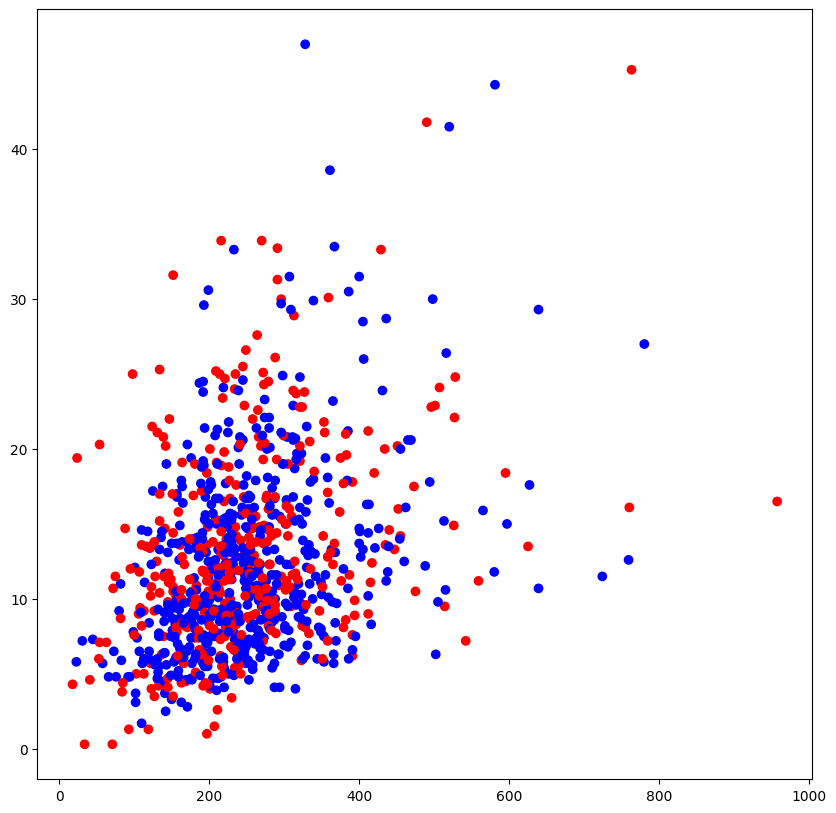
\includegraphics[width=\linewidth]{Figure/tabpfn-plt-wbc.png}
        \caption{Feature relation of plt and wbc}
        \label{fig:tabpfn-plt-wbc}
    \end{subfigure}
    \hfill
    \begin{subfigure}{0.45\textwidth}
        \centering
        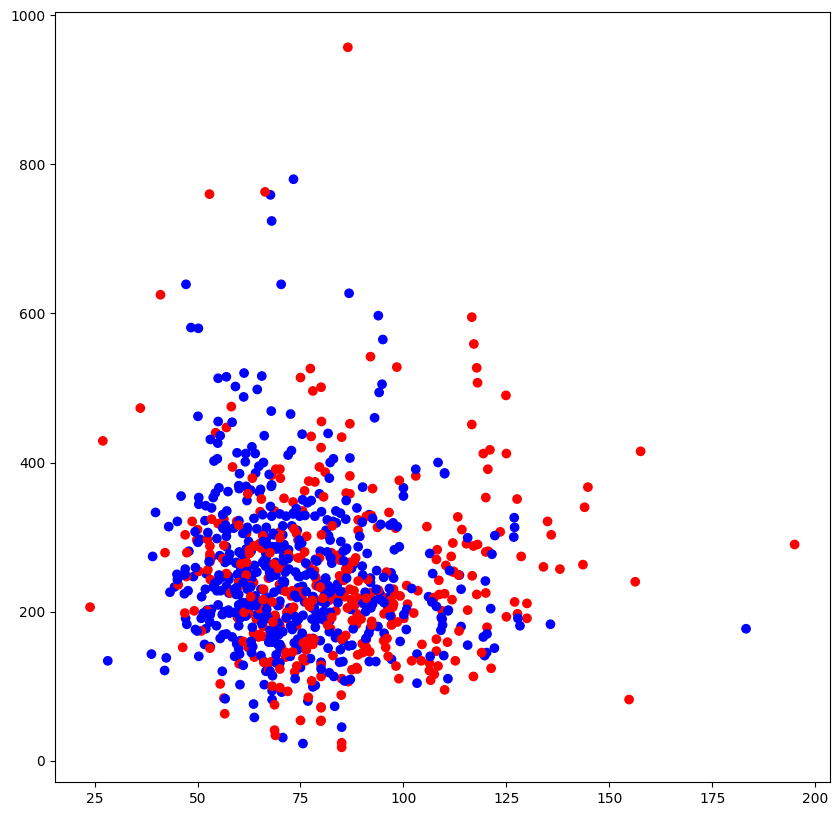
\includegraphics[width=\linewidth]{Figure/tabpfn-weight-plt.png}
        \caption{Feature relation of weight and plt}
        \label{fig:tabpfn-weight-plt}
    \end{subfigure}

    \vfill

    \begin{subfigure}{0.45\textwidth}
        \centering
        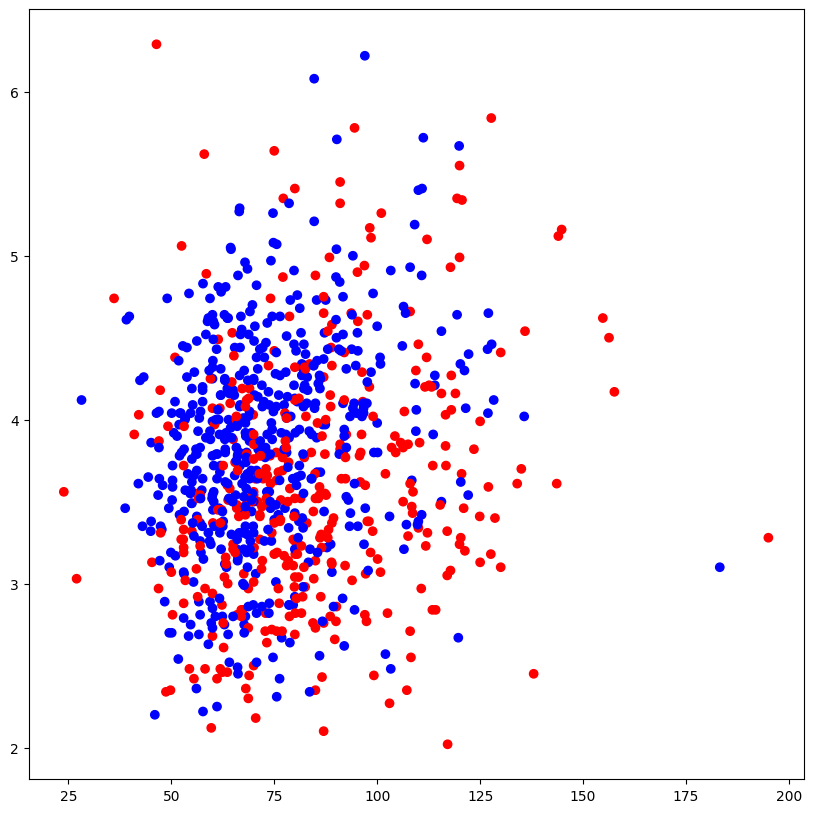
\includegraphics[width=\linewidth]{Figure/tabpfn-weight-rbc.png}
        \caption{Feature relation of weight and rbc}
        \label{fig:tabpfn-weight-rbc}
    \end{subfigure}
    \hfill
    \begin{subfigure}{0.45\textwidth}
        \centering
        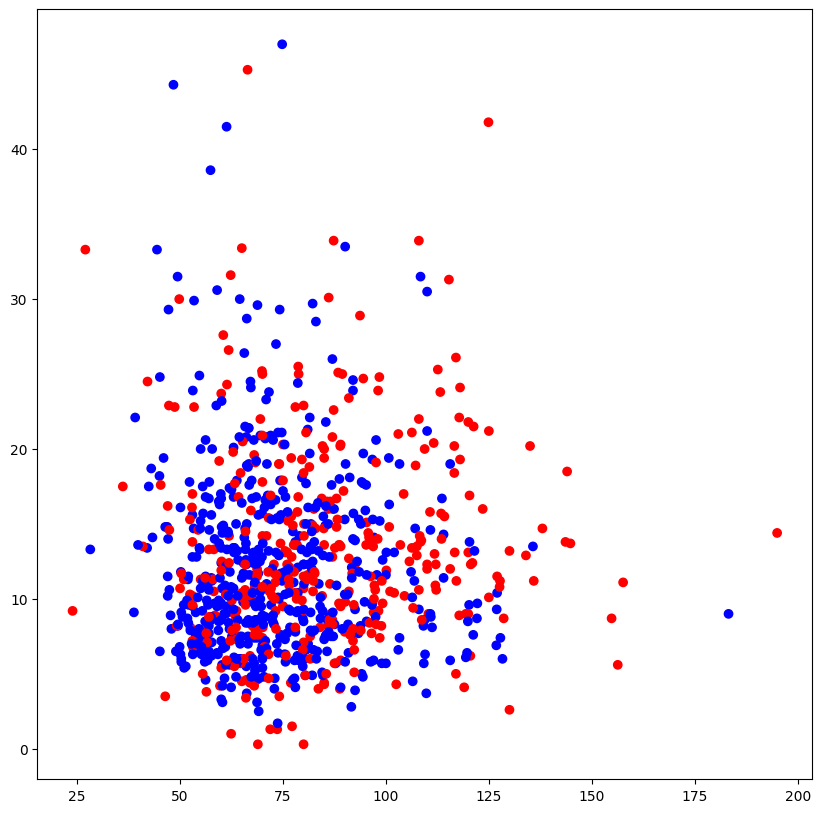
\includegraphics[width=\linewidth]{Figure/tabpfn-weight-wbc.png}
        \caption{Feature relation of weight and wbc}
        \label{fig:tabpfn-weight-wbc}
    \end{subfigure}

    \caption{Feature relation of TabPFN model}
    \label{fig:tabpfn-feature-relation}
\end{figure}


\section{Time series-based model}

In this section, I will describe the time series-based model used to predict the risk of Acute Kidney Injury in Diabetic Ketoacidosis patients.
The model is built using Tensorflow and Keras, it used a Long Short-Term Memory (LSTM) network to learn the temporal dependencies of time dependent features.

It starts the same with tabular-based models where the dataset is split into 5 parts and the model is trained on 4 parts and evaluated on the remaining part.
Instead of trying to predict the risk of AKI in DKA patients in a long time range of 7 days, this model expects to get patient's monitored status continuously and predict the risk of AKI in the next 24 hours.
That is why dynamic features' values are extracted in a time window of 1, 2, 3, 4, 6, 12, and 24 hours from the patient's intime up until the time of prediction.
The patients who are feasible to attend are the one who has not developed AKI from the beginning of the ICU stay to the time of prediction.
These values are then merged into a vector and fed into the LSTM network.
The static features are also extracted and fed into the network as a separate input.
The model is then trained to predict if the patient will develop AKI in the next 24 hours.

Here I will define two types of time windows that will be used in training: the predicting window and the feature window.
The predicting window is the time window from patient admission to the time of prediction.
The feature window is the time window with length of 1, 2, 3, 4, 6, 12, and 24 hours.
These windows are placed continuously in the predicting window.
Given LPW is the length of the predicting window and LFW is the length of the feature window, the number of feature windows in the predicting window is $LPW \div LFW$.

Since some patients have longer ICU stays than others, I shifted the predicting window in order to retain more training data.
For example, if a patients develop AKI after 6 days in the ICU, and the predicting window is 3 days, I will resampled this patient as three time windows: the first one is from the intime to 3 days after the intime, the second one is from 2 days after the intime to 4 days after the intime, and the last one is from 3 days after the intime to 5 days after the intime. 
This way, I can attained more training data and the model can learn the temporal dependencies of the features more effectively.

The model is then evaluated on the test set to determine the best length for feature window and predicting window.
The best model will then be compared to the tabular-based models to determine the best model for predicting the risk of Acute Kidney Injury in DKA-ICU patients.


\end{document}